\subsection{Projektbeschreibung}

Ziel dieses Projekts ist es, das Integral von Funktionen $f : \Omega \to \R$ für ein gegebenes Gebiet $\Omega \subset \R^2$ zu approximieren. Eine mögliche Strategie besteht darin, das Gebiet in disjunkte einfache Teilgebiete $T_i, i \in I$ für eine Indexmenge $I$ zu zerlegen, sodass
\begin{align*}
\Omega = \sum_{i \in I}{T_i}.
\end{align*}

Nun konstruiert man Quadraturformeln für die einfacheren Teilgebiete $T_i$ und summiert über die gebietweisen Integrale. Eine häufige Wahl für $T_i$ sind Dreiecke, deshalb konstruieren wir zunächst Integrationsregeln für das Einheitsdreieck. Sei $\hat{Q} := (0, 1) \times (0, 1)$ und $\hat{T}$ das offene Dreieck mit den Eckpunkten $(0, 0), (1, 0), (0, 1)$. Sei weiters

\begin{align*}
    \Psi:
    \begin{cases}
        \R^2    \to     \R^2        \\
        (x, y)  \mapsto (x, (1-x)y).
    \end{cases}
\end{align*}

\subsection{Vorüberlegungen}

Zuerst stellen wir fest, dass die Abbildung $\Psi$ ein Diffeomorphismus von $\R^2$ nach $\R^2$ ist: Wir betrachten die Funktionalmatrix
$\mathrm{d}\Psi =
                \left(\begin{array}{cccc}                                
                1 & 0  \\                                               
                -y & 1-x  \\
                \end{array}
                \right) $
 und erhalten aus der Stetigkeit der partiellen Ableitungen $\Psi \in \mathrm{C^{1}}$.
 
 
 Andererseits ist $\Psi^{-1}: (x, y) \mapsto \left( x, \frac{y}{1-x} \right)$ die Inverse von $\Psi$. Aus $\mathrm{d}\Psi^{-1} =
    \left(\begin{array}{ccccc}                                
                1 & 0  \\                                               
                \frac{y}{1-x^2} & \frac{1}{1-x}  \\
                \end{array}
                \right)$ schließen wir analog $\Psi^{-1} \in \mathrm{C^{1}}$.
 
 
 Für ein beliebiges $(x, y) \in \hat{Q}$ gibt es positive Zahlen $\epsilon_{x}$ und $\epsilon_{y}$ mit $x = 1 - \epsilon_{x}$ und $y = 1 - \epsilon_{y}$, damit gilt $\Psi(x,y) = (1 - \epsilon_{x}, \epsilon_{x} - \epsilon_{x} \epsilon_{y})$. Ein Punkt im ersten Quadranten liegt genau dann in $\hat{T}$, wenn die Summe seiner Komponenten kleiner als 1 ist. Es gilt $(1 - \epsilon_{x})+(\epsilon_{x} - \epsilon_{x} \epsilon_{y}) = 1 - \epsilon_{x}\epsilon_{y} < 1$ und damit $\Psi(\hat{Q}) \subseteq \hat{T}$.
 
Sei umgekehrt $(x, y) \in \hat{T}$, dann gilt $x + y < 1$. Dieser Punkt hat unter $\Psi$ das Urbild $\left(x, \frac{y}{1-x}\right)$. Aus $\frac{y}{1-x} < 1 \Leftrightarrow x + y < 1$ folgt $\Psi(\hat{Q}) \supseteq \hat{T}$ und somit insgesamt $\Psi(\hat{Q}) = \hat{T}$.

Also ist $\Psi$ auch ein Diffeomorphismus von $\hat{Q}$ nach $\hat{T}$.
\newline
\newline
\newpage
\subsection{Quadraturformeln auf $\hat{Q}$ und $\hat{T}$}
Für $N, M \in \N$ seien $Q_{N} = \sum_{j=0}^{n(N)}\alpha_{j}f(x_{j})$ und $Q_{M} = \sum_{j=0}^{n(M)}\beta_{j}f(y_{j})$ zwei Quadraturformeln der Ordnung $N+1$ bzw. $M+1$ auf dem Einheitsintervall. Wir definieren daraus auf $\hat{Q}$ eine Quadraturformel durch \begin{align*}{Q_{\hat{Q}} := \sum_{i=0}^{n(N)}\sum_{j=0}^{n(M)}\alpha_{i}\beta_{j}f(x_{i},y_{j}).}
\end{align*}



$\Pi_{N,M}$ sei der Raum aller Linearkombinationen von Polynomen der Form $p_{ij}: (x,y) \mapsto x^i y^j$ mit $i \leq N, j \leq M$.
Durch die Quadraturformel $Q_{\hat{Q}}$ werden alle Polynome aus $\Pi_{N,M}$ exakt integriert, denn es gilt für beliebiges $r \in \Pi_{N,M}$

\begin{align*}
    Q_{\hat{Q}}(r) &= \sum_{i=0}^{n(N)}\alpha_{i}\sum_{j=0}^{n(M)}\beta_{j}r(x_{i},y_{j}) \stackrel{(1)}{=} \sum_{i=0}^{n(N)}\alpha_{i}\int_{0}^{1}r(x_{i},y)~dy \\
    &= \int_{0}^{1}\sum_{i=0}^{n(N)}\alpha_{i}r(x_{i},y)~dy \stackrel{(2)}{=} \int_{0}^{1}\int_{0}^{1}r(x,y)~dxdy,
\end{align*}
wobei (1) [(2)] gilt, da $r(x_{i}, y)$ [$r(x,y)$] als Funktion in Abhängigkeit von $y$ [$x$] ein Polynom vom Grad $\leq M$ [$\leq N$] ist und daher durch $Q_{M}$ [$Q_{N}$] exakt integriert wird.
\newline
\newline
Mithilfe von $Q_{\hat{Q}}$ können wir nun auch eine Quadraturformel auf dem Einheitsdreieck $\hat{T}$ konstruieren: Wir definieren
\begin{align*}Q_{\hat{T}}(f) := Q_{\hat{Q}}((f\circ\Psi)|{\mathrm{det}(\mathrm{d}\Psi)}|)
\end{align*} und erhalten für $f$ mit $(f\circ\Psi)|\mathrm{det}(\mathrm{d}\Psi)| \in \Pi_{N,M}$
unter Verwendung der bereits gezeigten Eigenschaften von $\Psi$ und der Transformationsformel

\begin{align*}
    Q_{\hat{T}}(f) = \int_{0}^{1}\int_{0}^{1}(f\circ\Psi)(x,y)|\det(\mathrm{d}\Psi
    \left(\begin{array}{rr}
    x \\
    y \\
    \end{array}\right)
    )|~dx~dy =\int_{\hat{Q}}(f\circ\Psi)|\mathrm{det}(\mathrm{d}\Psi)|~d\lambda^{2} = \int_{\Psi(\hat{Q}) = \hat{T}} f~d\lambda^{2}.
\end{align*}
Die Polynome f, die durch $Q_{\hat{T}}$ exakt integriert werden, sind genau jene, die sich als Linearkombination von $p_{ij}: (x,y) \mapsto x^i y^j$ mit $i+j+1\leq N, j \leq M$ darstellen lassen. Für diese Basispolynome gilt nämlich
\begin{align*}
    (p_{ij}\circ\Psi)
    \left(\begin{array}{rr}
    x \\
    y \\
    \end{array}\right)
    |\det(\mathrm{d}\Psi
    \left(\begin{array}{rr}
    x \\
    y \\
    \end{array}\right)
    )| &= x^{i}(y-xy)^{j}|1-x| \\
    &= x^{i}(y^{j}+\dots\pm x^{j}y^{j})(1-x) \\
    &= x^{i}y^{j}+\dots\pm x^{i+j}y^{j} - x^{i+1}y^{j}+\dots\pm x^{i+j+1}y^{j}.
\end{align*}
\newline

\subsubsection{Gaußquadraturen}
Um Quadraturformeln auf dem Einheitsquadrat bzw. auf dem Einheitsdreieck anzugeben, die aus dem Produkt von Gauß-Quadraturen entstehen, müssen zunächst die Gauß-Quadraturen zur Gewichtsfunktion $\omega \equiv 1$ auf dem Einheitsintervall bestimmt werden.

Die zugehörigen Quadraturknoten auf dem Intervall $[-1,1]$ lassen sich mithilfe der Orthogonalpolynome bestimmen, die durch die Rekursion
\begin{align*}
    L_{0}(x) = 1,~~~~L_{1}(x)=x,~~~~L_{n+1}(x) = xL_{n}(x)-\frac{n^{2}}{4n^{2}-1}L_{n-1}(x),~~~~n \in \N
\end{align*}
gegeben sind.

Gemäß Satz 4.23 des Skripts sind die Nullstellen des $n$-ten Orthogonalpolynoms $L_{n}$ (und somit die $n$ Quadraturknoten der Gauß-Quadratur $Q_{n-1}$) genau die Eigenwerte der Matrix\newline
$
\left(\begin{array}{cccccc}                                
                \beta_{0} & \gamma_{1} &&& \\               \gamma_{1} & \beta_{1} & \gamma_{2} && \\
                & \gamma_{2} & \ddots & \ddots && \\
                && \ddots & \ddots & \gamma_{n-1} \\
                &&& \gamma_{n-1} & \beta_{n-1}
                \end{array}
                \right)$, wobei in unserem Fall für alle $m \in \N_{0}$ gilt $\beta_{m}=0, \gamma_{m}=\sqrt{\frac{m^{2}}{4m^{2}-1}}.$
                
                
Die affin-lineare Abbildung 
$
    \Phi : [-1,1] \to [0,1] : \zeta \mapsto \frac{1}{2}(1+\zeta)
$
liefert die entsprechenden Quadraturknoten auf dem Einheitsintervall.

Die zugehörigen Gewichte $\alpha_{j}$ werden ebenso wie in Satz 4.23 berechnet, wobei für normierte Eigenvektoren aus $\int_{0}^{1}\omega(x) = 1$ folgt, dass
\begin{align*}
    \alpha_{j} = ((v_{j})_{1})^{2},~~j = 0,\dots,n.
\end{align*}

\lstset{language=Python}
\lstset{frame=lines}
\lstset{caption={Berechnung von Knoten und Gewichten für die Gauß-Quadratur}}
\lstset{label={lst:code_direct}}
\lstset{basicstyle=\footnotesize}
\begin{lstlisting}
def nodesnweights(n): 

    gamma = np.array([np.sqrt((i+1)**2/(4*(i+1)**2-1)) for i in range(n-1)])
    T = np.zeros((n,n)) + np.diag(gamma,1) + np.diag(gamma,-1)
    [vals,vecs] = np.linalg.eig(T)  #vecs sind bereits normiert
    
    vals = phi(vals)
    alpha = np.array([(vecs[0][i])**2 for i in range(n)]) 
    return [vals,alpha] 
\end{lstlisting}
\hspace{10pt}

Die aus dem Produkt von solchen Gauß-Quadraturen entstehenden Quadraturformeln $Q_{\hat{Q}}$ und $Q_{\hat{T}}$ kann man nun analog zur Beschreibung von oben implementieren:


\lstset{language=Python}
\lstset{frame=lines}
\lstset{caption={Implementierung von $\mathrm{Q_\hat{Q}}$}}
\lstset{label={lst:code_direct}}
\lstset{basicstyle=\footnotesize}
\begin{lstlisting}
def gaussQ(f,n):
    [x,a] = nodesnweights(n+1)
    sum = 0
    for i in range(n+1):
        for j in range(n+1):
          sum += a[i]*a[j]*f(x[i],x[j])
    return sum
\end{lstlisting}


\lstset{language=Python}
\lstset{frame=lines}
\lstset{caption={Implementierung von $\mathrm{Q_\hat{T}}$}}
\lstset{label={lst:code_direct}}
\lstset{basicstyle=\footnotesize}
\begin{lstlisting}
def gaussUT(f,n):
    def z(x,y):
        return f(x,(1-x)*y)*(1-x)
    return gaussQ(z,n)
\end{lstlisting}

\newline
\subsubsection{Quadraturen auf $\hat{T}$ mithilfe von Lagrange-Polynomen}
Alternativ dazu konstruieren wir uns Quadraturformeln $Q_{n}(f) := \int_{\hat{T}}p_{f}~d\lambda^{2}$ auf dem Einheitsdreieck, wobei wir das interpolierende Polynom mit den in Übungsaufgabe 22 berechneten Lagrange-Polynomen darstellen können. Wie im eindimensionalen Fall erhalten wir also eine Quadraturformel der Form $Q_{n}(f) =~\sum_{j=0}^{n}\alpha_{j}f(x_{j}, y_{j})$ mit Quadraturgewichten $\alpha_{j}=\int_{\hat{T}}L_{j}(x,y)~d\lambda^{2}$.

\lstset{language=Python}
\lstset{frame=lines}
\lstset{caption={Quadraturformeln erster und zweiter Ordnung auf $\mathrm{\hat{T}}$} mit Lagrange-Polynomen}
\lstset{label={lst:code_direct}}
\lstset{basicstyle=\footnotesize}
\begin{lstlisting}
def interp1UT(f):
    z = [f(0,0),f(1,0),f(0,1)]
    return z[0]*(1/6) + z[1]*(1/6) + z[2]*(1/6)

def interp2UT(f):
    z = [f(0,0),f(1,0),f(0,1),f(1/2,1/2),f(1/2,0),f(0,1/2)]
    return z[0]*0 + z[1]*0 + z[2]*0 + z[3]*(1/6) + z[4]*(1/6) + z[5]*(1/6)
\end{lstlisting}
\newline
\newline

\subsection{Quadraturformeln auf beliebigen Dreiecken}
Nun können wir die bisher konstruierten Quadraturformeln auf dem Einheitsdreieck auch für ein beliebiges Dreieck $T$ verallgemeinern. Für ein solches Dreieck (gegeben durch die 3 affin unabhängigen Eckpunkte $x,y$ und $z$) definieren wir uns die affine Abbildung
\begin{align*}
    \pi_{T}: \hat{T} \to T : a \mapsto A_{T}(a) + x, \text{~~~~wobei~} A_{T} = \left(\begin{array}{cc}                                
                z_{1}-x_{1} & y_{1}-x_{1}  \\
                z_{2}-x_{2} & y_{2}-x_{2}  \\
                \end{array}
                \right). 
\end{align*}
Man kann leicht nachprüfen, dass diese Abbildung die drei Eckpunkte des Einheitsdreiecks auf $x$, $y$ und $z$ abbildet und somit $\pi_{T}(\hat{T}) = T$ leistet. 

Da A regulär ist, ist $\pi$ ein Diffeomorphismus und es gilt mit der Transformationsformel
\begin{align*}
    \int_{T}f~d\lambda^{2} = \int_{\pi_{T}(\hat{T})}f~d\lambda^{2} = \int_{\hat{T}}(f\circ\pi_{T})|\det(\mathrm{d}\pi_{T})|~d\lambda^{2}.
\end{align*}
Wir definieren also für eine auf dem Einheitsdreieck gegebene Quadraturformel $Q_{\hat{T}}$ die neue Quadraturformel auf $T$ als
\begin{align*}
    Q_{T}(f) :=  Q_{\hat{T}}((f\circ\pi_{T})|\det(\mathrm{d}\pi_{T})|) = Q_{\hat{T}}((f\circ\pi_{T})|\mathrm{det}(A_{T})|).
\end{align*}

\lstset{language=Python}
\lstset{frame=lines}
\lstset{caption={Gauß-Quadratur auf beliebigem Dreieck T}}
\lstset{label={lst:code_direct}}
\lstset{basicstyle=\footnotesize}
\begin{lstlisting}
def gaussT(f,n,T):
    def w(x,y):
        A = np.array([ [T[2][0]-T[0][0], T[1][0]-T[0][0]],
                       [T[2][1]-T[0][1], T[1][1]-T[0][1]] ])
        l = A@np.array([x,y]) + np.array([T[0][0],T[0][1]])
        det = abs(A[0][0]*A[1][1] - A[0][1]*A[1][0])
        return f(l[0],l[1])*det
    return gaussUT(w,n)
\end{lstlisting}

\lstset{language=Python}
\lstset{frame=lines}
\lstset{caption={Quadratur mit Lagrange-Polynomen auf beliebigem Dreieck T}}
\lstset{label={lst:code_direct}}
\lstset{basicstyle=\footnotesize}
\newpage
\begin{lstlisting}
def interp1T(f,T):
    def w(x,y):
        A = np.array([ [T[2][0]-T[0][0], T[1][0]-T[0][0]],
                       [T[2][1]-T[0][1], T[1][1]-T[0][1]] ])
        l = A@np.array([x,y]) + np.array([T[0][0],T[0][1]])
        det = abs(A[0][0]*A[1][1] - A[0][1]*A[1][0])
        return f(l[0],l[1])*det
    return interp1UT(w)


def interp2T(f,T):
    def w(x,y):
        A = np.array([ [T[2][0]-T[0][0], T[1][0]-T[0][0]],
                       [T[2][1]-T[0][1], T[1][1]-T[0][1]] ])
        l = A@np.array([x,y]) + np.array([T[0][0],T[0][1]])
        det = abs(A[0][0]*A[1][1] - A[0][1]*A[1][0])
        return f(l[0],l[1])*det
    return interp2UT(w)
\end{lstlisting}
\subsection{Quadraturformeln auf einem beliebigen Gebiet mithilfe von Triangulierung}
Jetzt sind wir fast am Ziel angelangt; wir betrachten nun ein Gebiet $\Omega \subset \R^2$ und eine Funktion $f : \Omega \to \R$. Unsere bisherige Arbeit liefert uns die Werkzeuge, um das Integral $\int_{\Omega}f~d\lambda^{2}$ näherungsweise zu berechnen. Hiezu betrachten wir disjunkte Dreiecke $T_i, i \in I$ mit $\sum_{i \in I}{T_i} \subseteq \Omega$. Es stellt sich die Frage, wie gut die Approximation
\begin{align*}
    \int_{\Omega}f~d\lambda^{2} \approx \sum_{i \in I}{Q_{T_{i}}(f)}
\end{align*}
in Abhängigkeit von der Feinheit der Triangulierung ist.\newline

Zuerst betrachten wir das Integral der Funktion $f: \R^2 \rightarrow \R, (x, y) \mapsto \mathrm{exp}(\frac{x+y}{x-y})$ über dem Viereck mit den Eckpunkten $(0, -1), (0, -2), (2, 0), (1, 0)$, das wir mithilfe der Transformationsformel exakt berechnen können. Wir verwenden das Python-Package $\mathrm{dmsh}$, um Triangulierungen zu generieren, wobei wir jeweils Dreiecke mit den Kantenlängen $h = (\frac{2}{3})^i, i = 1, ..., 10$ wählen. Dabei integrieren wir auf zwei Arten: Mit der aus dem Produkt von Gauß-Quadraturen konstruierten Formel $Q_{T}$ mit Ordnung 4 und mit der mithilfe von Lagrange-Interpolation konstruierten Quadraturformel 2. Ordnung. In diesem Test erweist sich letztere als mindestens ebenbürtig und liefert für $i \ge 7$ sogar einen besseren Schätzwert für das Integral. Mithilfe einer Vergleichsgerade können wir auf einem doppelt logarithmischen Plot ablesen, dass beide Formeln ungefähr Konvergenzordnung 4 haben (Abb. 1).
\newline \newline
Als nächstes testen wir unsere Formeln, indem wir die Funktion $g: \R^2 \rightarrow \R, (x, y) \mapsto \mathrm{sin}(x^2+y^2)$ über den Einheitskreis integrieren. Auch hier lässt sich der exakte Wert sofort über die Transformationsformel bestimmen. Aus dem Konvergenzplot (Abb. 2) schließen wir auf Konvergenzordnung 2. Der Fehler im ersten Beispiel war vergleichsweise klein und kann auf die Fehler der Quadraturformeln zurückgeführt werden; hier hingegen wird die Abhängigkeit von der Triangulierung deutlich, die ein rundes Gebiet nicht vollständig überdecken kann. Der dadurch entstandene Fehler ist so groß, dass er die Ungenauigkeit der Quadraturformeln verdeckt und kein Unterschied zwischen den beiden mehr ausgemacht werden kann.

\begin{center}
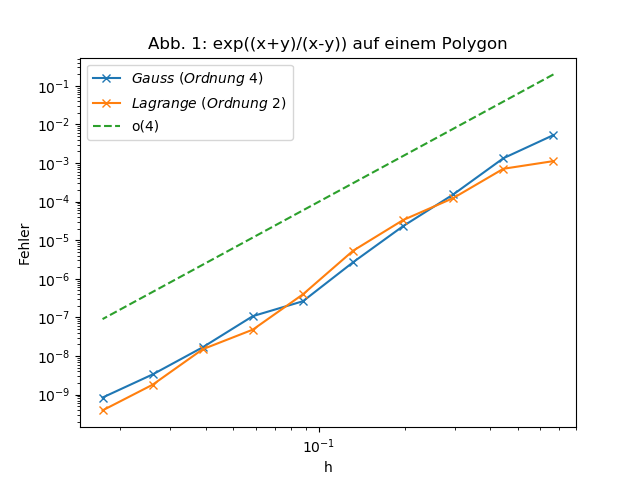
\includegraphics[width=120mm]{Aufgabe_3/Abb1.png}
\end{center}

\begin{center}
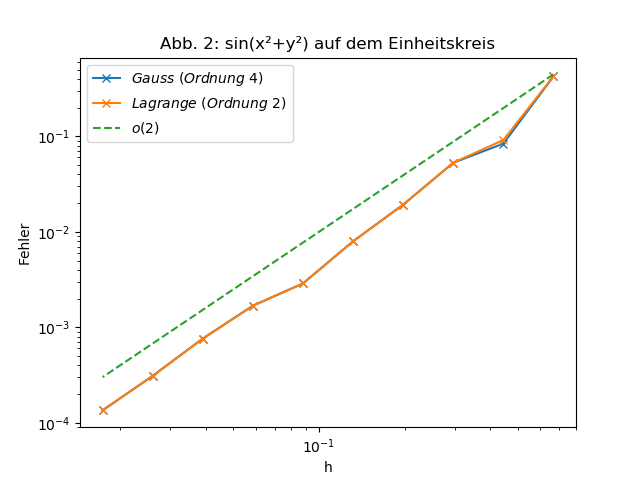
\includegraphics[width=120mm]{Aufgabe_3/Abb2.png}
\end{center}